\documentclass{beamer}

\usepackage{tikz}
\usetikzlibrary{positioning,matrix, arrows.meta}
\usetikzlibrary{graphdrawing.trees}
\usetikzlibrary{external}
\tikzexternalize % activate!
\usepackage{color}
\newcommand{\vet}[1]{\foreach \num in {#1}{\el{\num}}}
\newcommand{\vetempty}[1]{\foreach \num in {#1}{\elempty{\num}}}
\newcommand{\el}[1]{\tikz{\node[font=\smaller, draw]{#1}}}
\newcommand{\elempty}[1]{\tikz{\node[font=\small, minimum size=1cm, draw=white, fill=white]{#1}}}
\newcommand{\bl}{\color{blue}}
\newcommand{\gr}{\color{gray}}
\newcommand{\re}{\color{red}}
\newcommand{\tcb}[1]{\textcolor{blue}{#1}}
\newcommand{\tcg}[1]{\textcolor{green}{#1}}
\newcommand{\tcr}[1]{\textcolor{red}{#1}}
\newcommand{\ar}{\tikz{\draw [->] (0,0) -- (0,0.4)}}
\newcommand{\nd}{\color{white!0}.}

\usepackage{beamerthemeSingapore}
\usepackage{graphicx}
%\usepackage{here}
\usepackage{url}
\usepackage[brazil]{babel}
\usepackage[T1]{fontenc}
\usepackage[utf8]{inputenc}
%\usepackage[tight,raggedright]{subfigure}
\usepackage{subfigure}
\usepackage[alf]{abntex2cite}
\usepackage{listings}
\usepackage{minted}
\usepackage{algorithm2e}
\usepackage{amsmath}
\usepackage{pdfpages}
% Please add the following required packages to your document preamble:
\usepackage{booktabs}
\usepackage{ragged2e}
\usepackage{etoolbox}
\usepackage{mathtools}
\usepackage{caption}
\usepackage{xmpmulti}

\tikzset{
  treenode/.style = {align=center, inner sep=0pt, text centered,
    font=\sffamily},
  arn_bf/.style = {treenode, rectangle, rounded corners=.8ex, black, font=\sffamily\bfseries, draw=black,fill=white, text width=3.5em, inner sep=2pt },% arbre rouge noir, noeud noir
  arn_rf/.style = {treenode, rectangle, rounded corners=.8ex, red, font=\sffamily\bfseries, draw=red,fill=white, text width=3.5em, inner sep=2pt },% arbre rouge noir, noeud noir
  arn_bt/.style = {treenode, rectangle, rounded corners=.8ex, black, font=\sffamily\bfseries, draw=black,fill=white, text width=2.5em, inner sep=2pt },% arbre rouge noir, noeud noir
  arn_rt/.style = {treenode, rectangle, rounded corners=.8ex, red, font=\sffamily\bfseries, draw=red,fill=white, text width=2.5em, inner sep=2pt },% arbre rouge noir, noeud noir
  arn_b/.style = {treenode, circle, black, font=\sffamily\bfseries, draw=black,
    fill=white, text width=1.5em},% arbre rouge noir, noeud noir
  arn_bl/.style = {treenode, circle, blue, font=\sffamily\bfseries, draw=black,
    fill=white, text width=1.5em},% arbre rouge noir, noeud noir
  arn_n/.style = {treenode, circle, white, font=\sffamily\bfseries, draw=black,
    fill=black, text width=1.5em},% arbre rouge noir, noeud noir
  arn_r/.style = {treenode, circle, red, draw=red, 
    text width=1.5em, very thick},% arbre rouge noir, noeud rouge
  arn_x/.style = {treenode, rectangle, draw=black,
    minimum width=0.5em, minimum height=0.5em}% arbre rouge noir, nil
}

\captionsetup[figure]{labelformat=empty,textfont=smaller}

\DeclarePairedDelimiter{\ceil}{\lceil}{\rceil}

\apptocmd{\frame}{}{\justifying}{} % Allow optional arguments after frame.

\AtBeginSection[]{
  \begin{frame}
  \vfill
  \centering
  \begin{beamercolorbox}[sep=8pt,center,shadow=true,rounded=true]{title}
    \usebeamerfont{title}\insertsectionhead\par%
  \end{beamercolorbox}
  \vfill
  \end{frame}
}

% TODO TODO TODO TODO TODO TODO TODO
\title{09 - Árvores Balanceadas}
\author{Prof. Alex Kutzke}
\date{Junho de 2021}

\begin{document}

% ==========================================
\begin{frame}
  \begin{center}
    % TODO TODO TODO TODO TODO TODO
    \large{Setor de Educação Profissional e Tecnológica}\\
    Tecnologia em Análise e Desenvolvimento de Sistemas\\
    \vspace{1cm}			
    \small{DS141 - Estruturas de Dados II}
  \end{center}
  \titlepage
  \small{
  \center Tradução adaptada dos slides presentes em [1]. Imagens e exemplos também retirados do mesmo material.

  [1] \url{https://algs4.cs.princeton.edu/lectures/keynote/23Quicksort.pdf}}
\end{frame}
% ==========================================

% ==========================================
\begin{frame}[c]{Roteiro}
  \tableofcontents

\end{frame}
% ==========================================

\section{Árvores 2-3}

\begin{frame}[c]{Revisão de Implementações de Tabela de Símbolos}
  \begin{figure}[h]
    \centering
    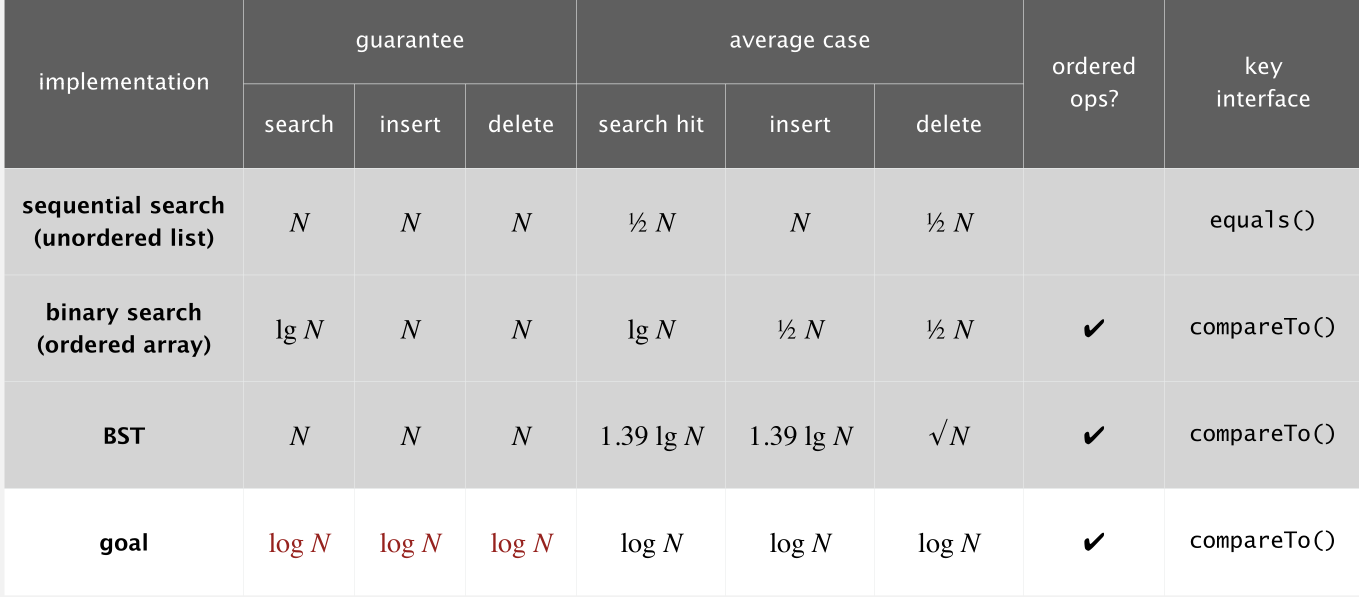
\includegraphics[width=\textwidth]{img/symbol_table_review.png}
    \caption{Fonte: \cite{sedgewick2014algorithms}}
  \end{figure}

  \begin{description}
    \item [Desafio] garantia de performance.
  \end{description}
\end{frame}

\begin{frame}
  \frametitle{Árvores 2-3}

  Permite \tcb{uma} ou \tcb{duas} chaves por nó:
  \begin{itemize}
    \item Nó-2: \textbf{uma chave}, \tcr{dois filhos};
    \item Nó-3: \textbf{duas chaves}, \tcr{três filhos};
  \end{itemize}

  \vspace{1cm}

  Propriedades:
  \begin{description}
    \item [Ordem simétrica] percurso in-ordem percorre as chaves em ordem crescente;
    \item [Balanceamento perfeito] Todos os caminhos da raiz até as folhas tem o mesmo comprimento;
  \end{description}

  \pause

  Como manter o balanceamento perfeito?

\end{frame}

\begin{frame}[c]{Exemplo: árvore 2-3}
  \begin{figure}[h]
    \centering
    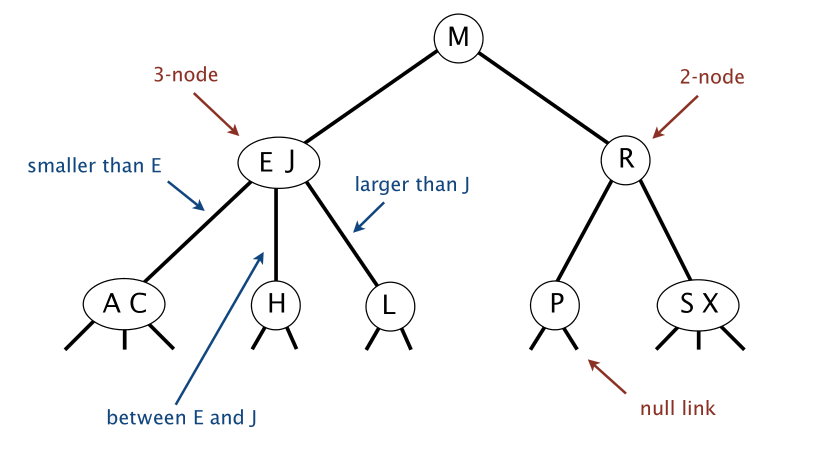
\includegraphics[width=\textwidth]{img/2_3_tree_example.png}
    \caption{Fonte: \cite{sedgewick2014algorithms}}
  \end{figure}
\end{frame}

\begin{frame}[t]
  \frametitle{Busca}

  \begin{enumerate}
    \item Compara o elemento buscado com as chaves da raiz;
    \item Encontra o intervalo que contém o elemento busca;
    \item Busca recursivamente através do filho associado ao intervalo;
  \end{enumerate}

  \only<2-5>{Busca por \tcr{H}}

    \vspace{1cm}
    \noindent
    \centering
    \begin{tikzpicture}[
        -, 
        level/.style={sibling distance=40mm/####1},
      ]
        \node (root) [arn_b] {M}
          child { 
            node (nEJ) [arn_bt] {E J} 
            child {
              node (nAC) [arn_bt] {A C} 
            }
            child {
              node (nH) [arn_b] {H} 
            }
            child {
              node (nL) [arn_b] {L} 
            }
          }
          child { 
            node (nR) [arn_b] {R} 
            child {
              node (nP) [arn_b] {P} 
            }
            child {
              node (nSX) [arn_bt] {S X} 
            }
          }
          ;
          \only<3>{\node [arn_r,  at = (root)] {M};}
          \only<4>{\node [arn_rt, at = (nEJ)] {E J};}
          \only<5>{\node [arn_r,  at = (nH)] {H};}
    \end{tikzpicture}

\end{frame}


\begin{frame}[t]
  \frametitle{Inserção}

  \tcb{Inserção em um nó-2 folha}
  \begin{enumerate}
    \item Adiciona chave a nó-2,  transformando-o em um nó-3;
  \end{enumerate}

  \only<2-6>{Inserir \tcr{G}}

    \vspace{1cm}
    \noindent
    \centering
    \begin{tikzpicture}[
        -, 
        level/.style={sibling distance=40mm/####1},
      ]
        \only<1-5>{
          \node (root) [arn_b] {L}
            child { 
              node (nE) [arn_b] {E} 
              child {
                node (nAC) [arn_bt] {A C} 
              }
              child {
                node (nH) [arn_b] {H} 
              }
            }
            child { 
              node (nR) [arn_b] {R} 
              child {
                node (nP) [arn_b] {P} 
              }
              child {
                node (nSX) [arn_bt] {S X} 
              }
            }
            ;
          }
          \only<3>{\node [arn_r,  above left=0pt of root] {G};}
          \only<4>{\node [arn_r,  above left=0pt of nE] {G};}
          \only<5>{\node [arn_r,  above left=0pt of nH] {G};}
        \only<6>{
          \node (root) [arn_b] {L}
            child { 
              node (nE) [arn_b] {E} 
              child {
                node (nAC) [arn_bt] {A C} 
              }
              child {
                node (nH) [arn_rt] {G H} 
              }
            }
            child { 
              node (nR) [arn_b] {R} 
              child {
                node (nP) [arn_b] {P} 
              }
              child {
                node (nSX) [arn_bt] {S X} 
              }
            }
            ;
          }
    \end{tikzpicture}

\end{frame}

\begin{frame}[t]
  \frametitle{Inserção}

  \tcb{Inserção em um nó-3 folha}
  \begin{enumerate}
    \item Adiciona chave a nó-3,  transformando-o em, temporariamente, um nó-4;
    \item Mova a chave intermediaria do nó-4 para o nó pai;
    \item Repita o processo na árvore acima se necessário;
    \item Se alcançar a raiz e esta se tornar um nó-4, dividir em 3 nós-2;
  \end{enumerate}

  \only<2-7>{Inserir \tcr{Z}}

    \noindent
    \centering
    \begin{tikzpicture}[
        -, 
        level/.style={sibling distance=40mm/####1},
      ]
        \only<1-5>{
          \node (root) [arn_b] {L}
            child { 
              node (nE) [arn_b] {E} 
              child {
                node (nAC) [arn_bt] {A C} 
              }
              child {
                node (nH) [arn_b] {H} 
              }
            }
            child { 
              node (nR) [arn_b] {R} 
              child {
                node (nP) [arn_b] {P} 
              }
              child {
                node (nSX) [arn_bt] {S X} 
              }
            }
            ;
          }
          \only<3>{\node [arn_r,  above left=0pt of root] {Z};}
          \only<4>{\node [arn_r,  above left=0pt of nR] {Z};}
          \only<5>{\node [arn_r,  above left=0pt of nSX] {Z};}
        \only<6>{
          \node (root) [arn_b] {L}
            child { 
              node (nE) [arn_b] {E} 
              child {
                node (nAC) [arn_bt] {A C} 
              }
              child {
                node (nH) [arn_b] {H} 
              }
            }
            child { 
              node (nR) [arn_b] {R} 
              child {
                node (nP) [arn_b] {P} 
              }
              child {
                node (nSX) [arn_rf] {S X Z} 
              }
            }
            ;
          }
        \only<7>{
          \node (root) [arn_b] {L}
            child { 
              node (nE) [arn_b] {E} 
              child {
                node (nAC) [arn_bt] {A C} 
              }
              child {
                node (nH) [arn_b] {H} 
              }
            }
            child { 
              node (nR) [arn_rt] {R X} 
              child {
                node (nP) [arn_b] {P} 
              }
              child {
                node (nS) [arn_b] {S} 
              }
              child {
                node (nZ) [arn_b] {Z} 
              }
            }
            ;
          }
    \end{tikzpicture}

\end{frame}


\begin{frame}[t]
  \frametitle{Exemplo: inserção}

  \only<1>{Inserir \tcr{S}}
  \only<2>{Inserir \tcr{X}}
  \only<3>{Inserir \tcr{H}}
  \only<4>{Inserir \tcr{R}}
  \only<5>{Inserir \tcr{A}}
  \only<6>{Inserir \tcr{P}}
  \only<7>{Inserir \tcr{E}}
  \only<8>{Inserir \tcr{C}}
  \only<9>{Inserir \tcr{L}}
  \only<10>{Resultado final:}

    \noindent
    \centering
    \begin{tikzpicture}[
        -, 
        level/.style={sibling distance=40mm/####1},
      ]
        \only<2>{
          \node [arn_b] {S} ;
        }
        \only<3>{
          \node [arn_bt] {S X} ;
        }
        \only<4>{
          \node [arn_b] {S} 
          child {
            node [arn_b] {H} 
          }
          child {
            node [arn_b] {X} 
          }
        ;}
        \only<5>{
          \node [arn_b] {S} 
          child {
            node [arn_bt] {H R} 
          }
          child {
            node [arn_b] {X} 
          }
        ;}
        \only<6>{
          \node [arn_bt] {H S} 
          child {
            node [arn_b] {A} 
          }
          child {
            node [arn_b] {R} 
          }
          child {
            node [arn_b] {X} 
          }
        ;}
        \only<7>{
          \node [arn_bt] {H S} 
          child {
            node [arn_b] {A} 
          }
          child {
            node [arn_bt] {P R} 
          }
          child {
            node [arn_b] {X} 
          }
        ;}
        \only<8>{
          \node [arn_bt] {H S} 
          child {
            node [arn_bt] {A E} 
          }
          child {
            node [arn_bt] {P R} 
          }
          child {
            node [arn_b] {X} 
          }
        ;}
        \only<9>{
          \node [arn_b] {H} 
          child {
            node [arn_b] {C} 
            child {
              node [arn_b] {A} 
            }
            child {
              node [arn_b] {E} 
            }
          }
          child {
            node [arn_b] {S} 
            child {
              node [arn_bt] {PR} 
            }
            child {
              node [arn_b] {X} 
            }
          }
        ;}
        \only<10>{
          \node [arn_b] {H} 
          child {
            node [arn_b] {C} 
            child {
              node [arn_b] {A} 
            }
            child {
              node [arn_b] {E} 
            }
          }
          child {
            node [arn_bt] {P S} 
            child {
              node [arn_b] {L} 
            }
            child {
              node [arn_b] {R} 
            }
            child {
              node [arn_b] {X} 
            }
          }
        ;}
    \end{tikzpicture}

\end{frame}

\begin{frame}
  \frametitle{Transformações locais}

  Dividir um \tcr{nó-4} temporário em um \tcb{nó-3} é uma \textbf{operação local}: \textit{número de operações necessárias é constante}.
  
  \begin{figure}[h]
    \centering
    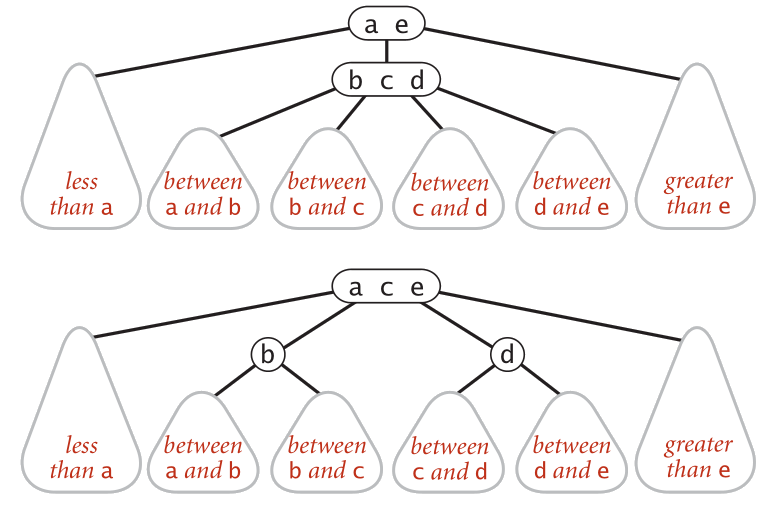
\includegraphics[width=.7\textwidth]{img/local_transformation.png}
    \caption{Fonte: \cite{sedgewick2014algorithms}}
  \end{figure}

\end{frame}

\begin{frame}
  \frametitle{Propriedades}

  \tcb{Invariantes:} Mantém ordem simétrica e balanceamento perfeito;


  \tcb{Por que?} Cada transformação mantém ordem simétrica e balanceamento perfeito;
  
  \begin{figure}[h]
    \centering
    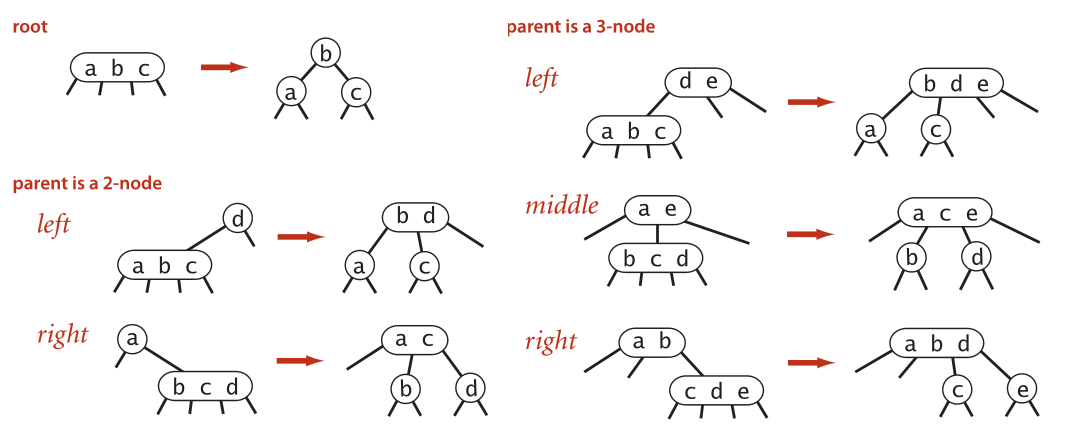
\includegraphics[width=\textwidth]{img/2_3_transformations.png}
    \caption{Fonte: \cite{sedgewick2014algorithms}}
  \end{figure}

\end{frame}

\begin{frame}
  \frametitle{Desempenho}

  \tcb{Balanceamento perfeito:} Todos os caminhos da raiz até as folhas tem o mesmo comprimento.
  \begin{figure}[h]
    \centering
    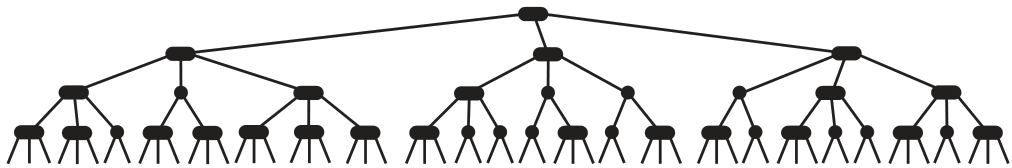
\includegraphics[width=\textwidth]{img/2_3_big.png}
    \caption{Fonte: \cite{sedgewick2014algorithms}}
  \end{figure}

  \tcb{Altura da árvore}
  \begin{itemize}
    \item Pior caso: $\log{N}$ \textcolor{gray}{- todos nós-2}
    \item Melhor caso: $\log_{3}{N} \sim .613 \lg{N}$ \textcolor{gray}{- todos nós-3}
    \item Entre 12 e 20 para \textbf{um milhão de nós};
    \item Entre 18 e 30 para \textbf{um bilhão de nós};
  \end{itemize}

  \tcb{Resumo} Desempenho \tcr{logarítmico} garantido para busca e inserção.

\end{frame}

\begin{frame}[c]{Sumário de Implementações de Tabela de Símbolos}
  \begin{figure}[h]
    \centering
    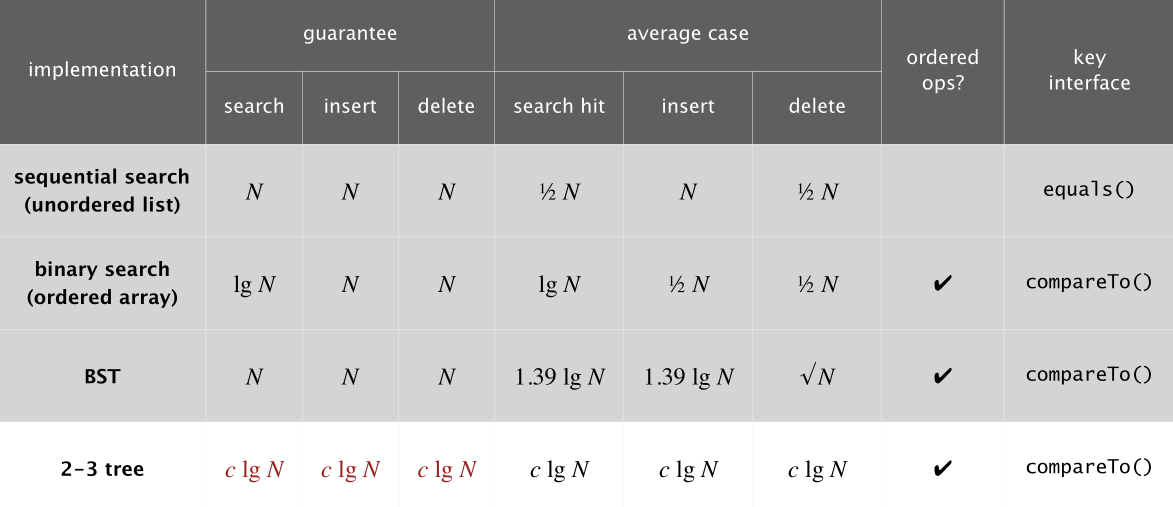
\includegraphics[width=\textwidth]{img/symbol_table_review_2.png}
    \caption{Fonte: \cite{sedgewick2014algorithms}}
  \end{figure}

  Constante \tcr{c} depende da implementação.
\end{frame}

\begin{frame}
  \frametitle{Implementação}

  \small
  \tcb{Implementação é complicada, porque:}
  \begin{itemize}
    \item Manter vários tipos de nós é trabalhoso;
    \item Várias comparações são necessárias para caminhar abaixo na árvore;
    \item A divisão de nós-4 temporários necessita percorrer a árvore para cima;
    \item Muitos casos diferentes para divisão de nós;
  \end{itemize}

  \begin{figure}[h]
    \centering
    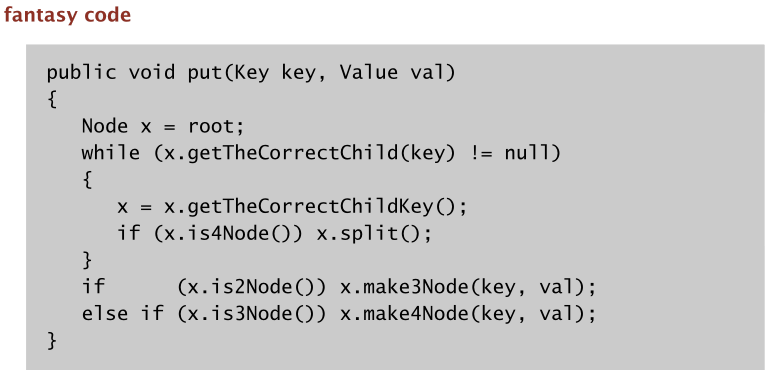
\includegraphics[width=.6\textwidth]{img/2_3_fantasy_code.png}
    \caption{Fonte: \cite{sedgewick2014algorithms}}
  \end{figure}

  \tcb{Resumo} Dá pra fazer, mas tem um jeito melhor. :)

\end{frame}

\section{Árvores Red-Black}

\begin{frame}[t]
  \frametitle{Como implementar Árvores 2-3 com Árvores Binárias?}

  \begin{columns}
    \small
    \begin{column}{0.85\textwidth}
  \tcb{Desafio} Como representar um nó-3?

  \vspace{1cm}
  
      \tcb{Abordagem 1: árvore binária simples}
      \begin{itemize}
        \item Sem forma de diferenciar um nó-3 de um nó-2;
        \item Impossível mapear uma árvore binária de volta e uma 2-3;
      \end{itemize}
      
      \tcb{Abordagem 2: árvore binária com nós ``cola''}
      \begin{itemize}
        \item Desperdiça espaço, desperdiça links;
        \item Código, provavelmente, confuso;
      \end{itemize}
      
      \tcb{Abordagem 3: árvore binária com arestas ``cola'' vermelhas}
      \begin{itemize}
        \item Bastante utilizado na prática;
        \item Restrição abstrata: arestas vermelhas descem para esquerda;
      \end{itemize}
    \end{column}
    \begin{column}{0.15\textwidth}
      \begin{figure}[h]
        \centering
        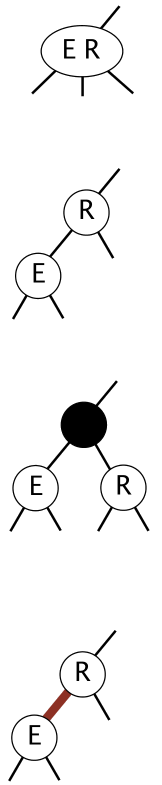
\includegraphics[height=.7\textheight]{img/2_3_to_bst.png}
      \end{figure}
    \end{column}
  \end{columns}

\end{frame}

\begin{frame}
  \frametitle{Árvores Left-leaning Red-black\\ \small{(Guibas-Sedgewick 1979 and Sedgewick 2007)}}

  \begin{enumerate}
    \item Representa árvores 2-3 com árvores binárias;
    \item Usa \tcr{arestas descendentes à esquerda} como ``cola'' para nós-3.
  \end{enumerate}
  
  \begin{figure}[h]
    \centering
    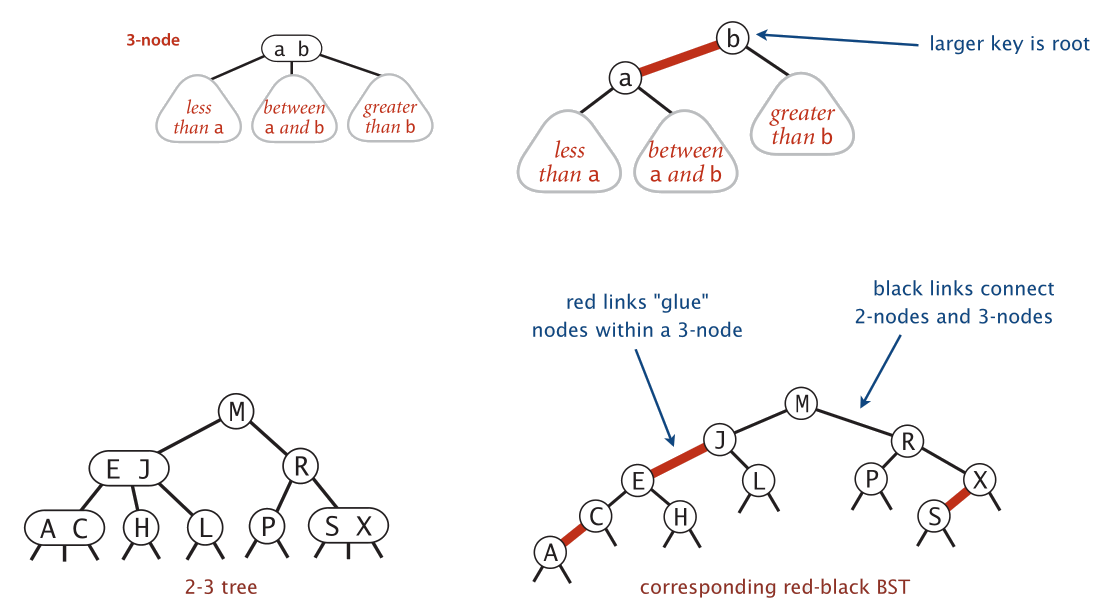
\includegraphics[width=.8\textwidth]{img/2_3_to_red_black.png}
    \caption{Fonte: \cite{sedgewick2014algorithms}}
  \end{figure}

\end{frame}

\begin{frame}
  \frametitle{Árvores Left-leaning Red-black: definição}

  Uma árvore binária tal que:
  \begin{itemize}
    \item Nenhum nó tem duas arestas vermelhas conectadas a si;
    \item Todos os caminhos da raiz até as folhas possuem o mesmo número de arestas pretas \textcolor{gray}{```balanceamento perfeito preto''};
    \item Arestas vermelhas sempre são descendentes à esquerda.
  \end{itemize}

  \begin{figure}[h]
    \centering
    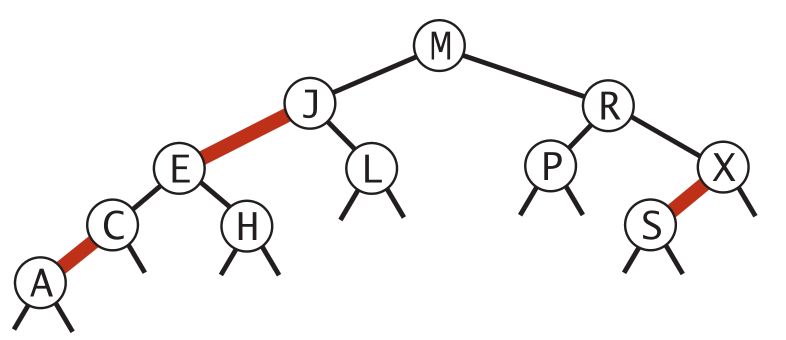
\includegraphics[width=.8\textwidth]{img/red_black_example.png}
    \caption{Fonte: \cite{sedgewick2014algorithms}}
  \end{figure}

\end{frame}

\begin{frame}
  \frametitle{Correspondência direta com Árvores 2-3}

  \tcb{Propriedade chave} Possui correspondência direta com árvores 2-3: 

  \begin{figure}[h]
    \centering
    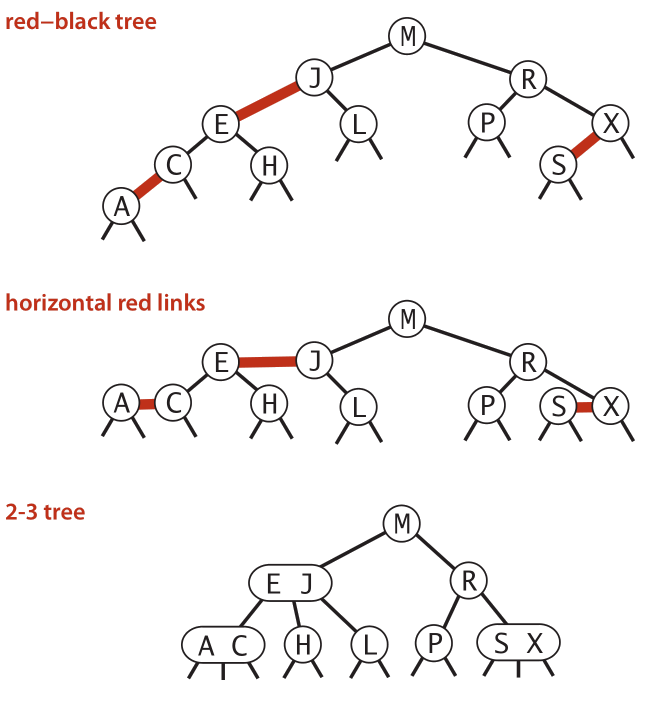
\includegraphics[width=.5\textwidth]{img/red_black_to_2_3.png}
    \caption{Fonte: \cite{sedgewick2014algorithms}}
  \end{figure}

\end{frame}

\begin{frame}
  \frametitle{Busca}

  Operação de busca é a mesma de Árvores Binárias Simples (basta ignorar a cor):
  \textcolor{gray}{Mas é mais rápido pois a árvore red-black tem um balanceamento melhor}

  \begin{figure}[h]
    \centering
    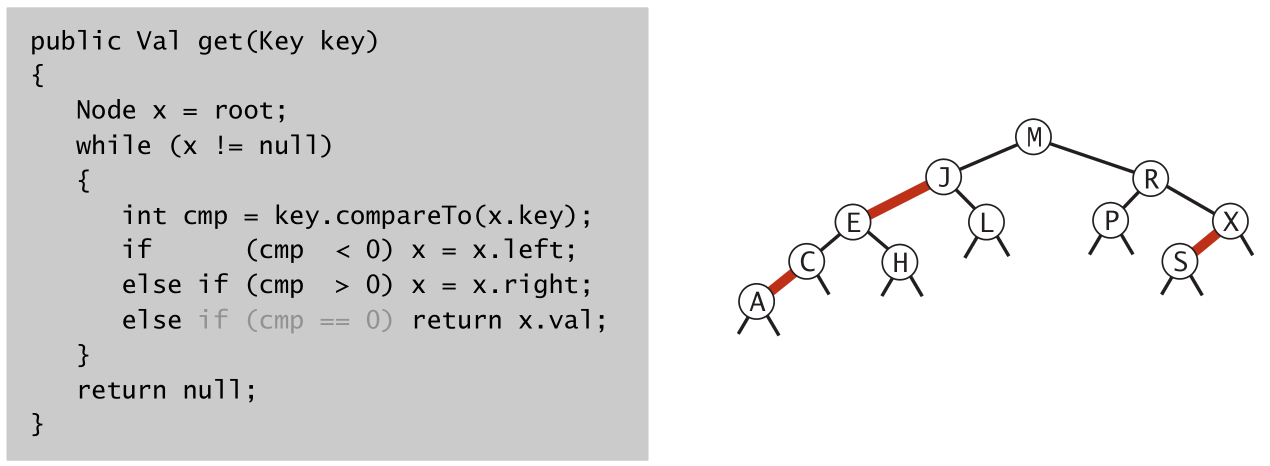
\includegraphics[width=\textwidth]{img/red_black_search.png}
    \caption{Fonte: \cite{sedgewick2014algorithms}}
  \end{figure}

  \tcb{Observação} Maior parte das outras operações também são idênticas.
\end{frame}

\begin{frame}[fragile]
  \frametitle{Representação}

  Informação da cor pode ser armazenada no nó filho da aresta.

      \begin{minted}[frame=lines,framesep=2mm,baselinestretch=1,fontsize=\normalsize,linenos,
        highlightlines={1,2,6,11-14}]{c}
#define RED    1
#define BLACK  0

typedef struct arvoreRB {
  int info;
  int cor;
  struct arvoreRB *esq;
  struct arvoreRB *dir;
} ArvoreRB;

int eh_no_vermelho(ArvoreRB * no){
  if(!no) return BLACK;
  return(no->cor == RED);
}
      \end{minted}
\end{frame}

\begin{frame}
  \frametitle{Representação: exemplo}

      \noindent
      \centering
      \begin{tikzpicture}[
          -, 
          level/.style={sibling distance=40mm/####1},
        ]
          \node (E) [arn_b] {E}
            child { 
              node (C) [arn_b] {C} 
              child {
                node (A) [arn_b] {A} 
              }
              child {
                node (D) [arn_b] {D} 
              }
            }
            child { 
              node (J) [arn_b] {J} 
              child {
                node (G) [arn_b] {G} 
              }
              child [missing]
            }
            ;
            \draw (E) -- (C) [red, very thick]; 
            \draw (J) -- (G) [red, very thick];
            \node (labelC) [left= 0.5cm of C, yshift=40, xshift=20, gray] {$\scriptstyle h.esq.cor == RED$};
            \draw[->,shorten <= 5pt, shorten >= 5pt,gray] (labelC) -- (C);
            \node (labelE) [above= 0.2cm of E, yshift=20, xshift=-20,gray] {\scriptsize h};
            \draw[->,shorten <= 5pt, shorten >= 5pt,gray] (labelE) -- (E);
            \node (labelJ) [above= 0.5cm of J, yshift=20, xshift=20, gray] {$\scriptstyle h.dir.cor == BLACK$};
            \draw[->,shorten <= 5pt, shorten >= 5pt,gray] (labelJ) -- (J);
      \end{tikzpicture}
  

\end{frame}

\begin{frame}
  \frametitle{Inserção Árvore RB}

  \tcb{Estratégia básica:} Manter correspondência direta com árvores 2-3.

  \tcb{Durante operações internas, manter:}
  \begin{itemize}
    \item Ordem simétrica;
    \item Balanceamento perfeito de arestas pretas;\\
          \textcolor{gray}{mas não necessariamente manter cores.}
  \end{itemize}
  
  \begin{figure}[h]
    \centering
    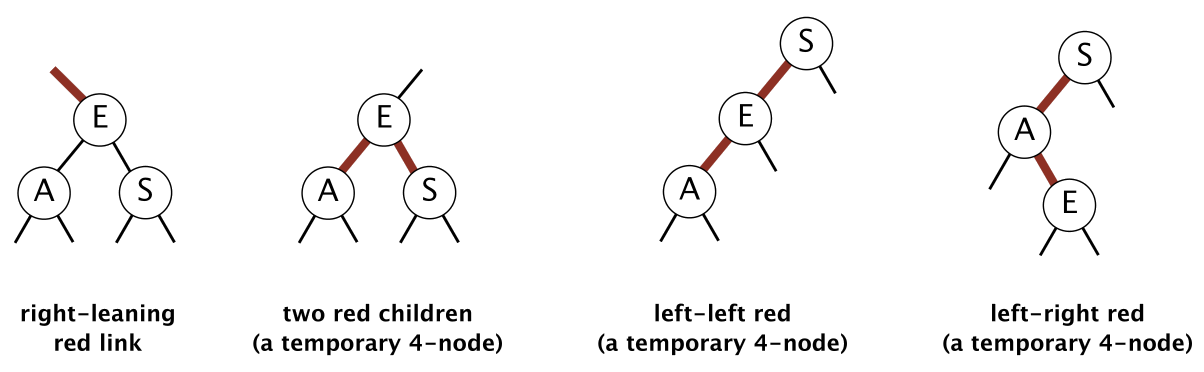
\includegraphics[width=.9\textwidth]{img/red_black_internal_operations.png}
    \caption{Fonte: \cite{sedgewick2014algorithms}}
  \end{figure}

  \tcb{Como?} Aplicar operações elementares de \textbf{rotação} e \textbf{troca de cor}.

\end{frame}

\begin{frame}[fragile,t]
  \frametitle{Operações elementares de Árvores RB}

  \tcb{Rotação à esquerda} Manter correspondência direta com árvores 2-3.

  \begin{columns}
    \begin{column}{0.5\textwidth}
      \begin{figure}[h]
        \centering
        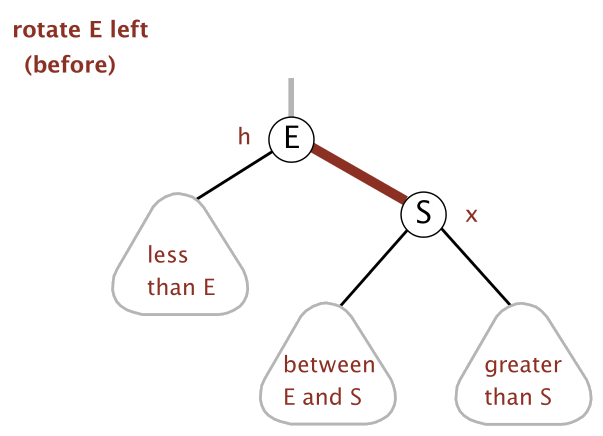
\includegraphics[width=.9\textwidth]{img/red_black_rot_left_before.png}
        \caption{Fonte: \cite{sedgewick2014algorithms}}
      \end{figure}
    \end{column}
    \begin{column}{0.5\textwidth}
      \begin{figure}[h]
        \centering
        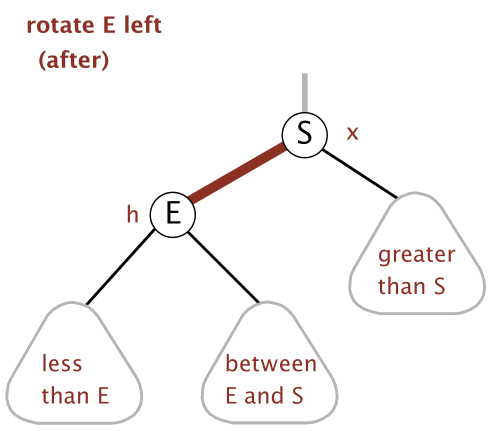
\includegraphics[width=.8\textwidth]{img/red_black_rot_left_after.png}
        \caption{Fonte: \cite{sedgewick2014algorithms}}
      \end{figure}
    \end{column}
  \end{columns}


  \tcb{Invariantes:} Manter ordem simétrica e balanceamento perfeito de arestas pretas.

\end{frame}

\begin{frame}[fragile,t]
  \frametitle{Operações elementares de Árvores RB}

  \tcb{Rotação à esquerda} Manter correspondência direta com árvores 2-3.

      \begin{minted}[frame=lines,framesep=2mm,baselinestretch=1,fontsize=\small,linenos]{c}
ArvoreRB * rot_esq(ArvoreRB * no){
  ArvoreRB * x = no->dir;
  no->dir = x->esq;
  x->esq = no;
  x->cor = no->cor;
  no->cor = RED;
  return(x);
}
      \end{minted}

  \tcb{Invariantes:} Manter ordem simétrica e balanceamento perfeito de arestas pretas.

\end{frame}

\begin{frame}[fragile,t]
  \frametitle{Operações elementares de Árvores RB}

  \tcb{Rotação à direita} Passar uma aresta vermelha temporariamente à direita.

  \begin{columns}
    \begin{column}{0.5\textwidth}
      \begin{figure}[h]
        \centering
        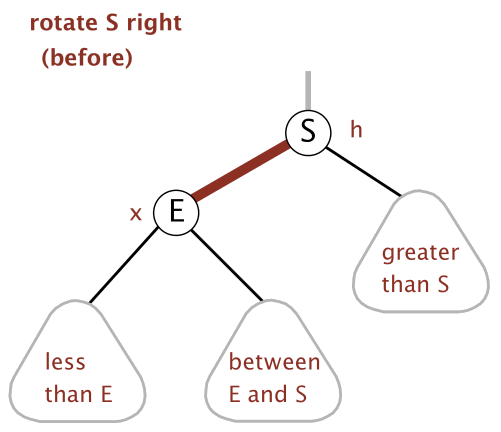
\includegraphics[width=.75\textwidth]{img/red_black_rot_right_before.png}
        \caption{Fonte: \cite{sedgewick2014algorithms}}
      \end{figure}
    \end{column}
    \begin{column}{0.5\textwidth}
      \begin{figure}[h]
        \centering
        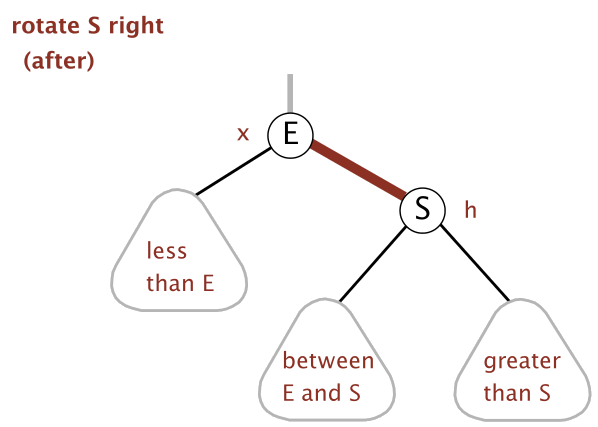
\includegraphics[width=.9\textwidth]{img/red_black_rot_right_after.png}
        \caption{Fonte: \cite{sedgewick2014algorithms}}
      \end{figure}
    \end{column}
  \end{columns}

  \tcb{Invariantes:} Manter ordem simétrica e balanceamento perfeito de arestas pretas.

\end{frame}

\begin{frame}[fragile,t]
  \frametitle{Operações elementares de Árvores RB}

  \tcb{Rotação à direita} Passar uma aresta vermelha temporariamente à direita.

      \begin{minted}[frame=lines,framesep=2mm,baselinestretch=1,fontsize=\small,linenos]{c}
ArvoreRB * rot_dir(ArvoreRB * no){
  ArvoreRB * x = no->esq;
  no->left = x->dir;
  x->dir = no;
  x->cor = no->cor;
  no->cor = RED;
  return(x);
}
      \end{minted}

  \tcb{Invariantes:} Manter ordem simétrica e balanceamento perfeito de arestas pretas.

\end{frame}

\begin{frame}[fragile,t]
  \frametitle{Operações elementares de Árvores RB}

  \tcb{Color flip} Recolorir um nó-4 temporário para dividi-lo.

  \begin{columns}
    \begin{column}{0.5\textwidth}
      \begin{figure}[h]
        \centering
        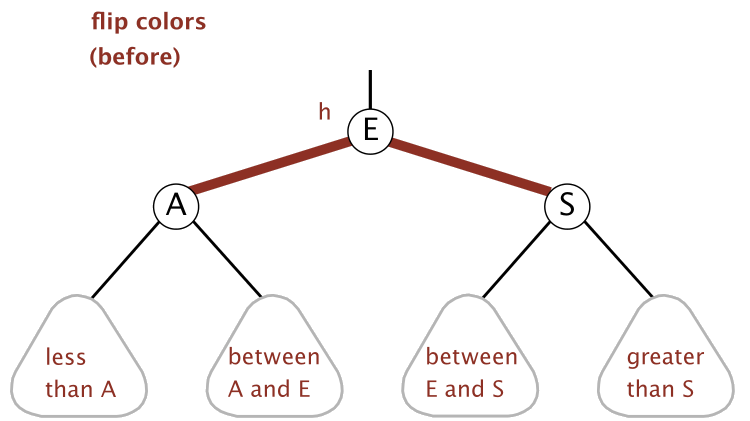
\includegraphics[width=.9\textwidth]{img/red_black_colo_flip_before.png}
        \caption{Fonte: \cite{sedgewick2014algorithms}}
      \end{figure}
    \end{column}
    \begin{column}{0.5\textwidth}
      \begin{figure}[h]
        \centering
        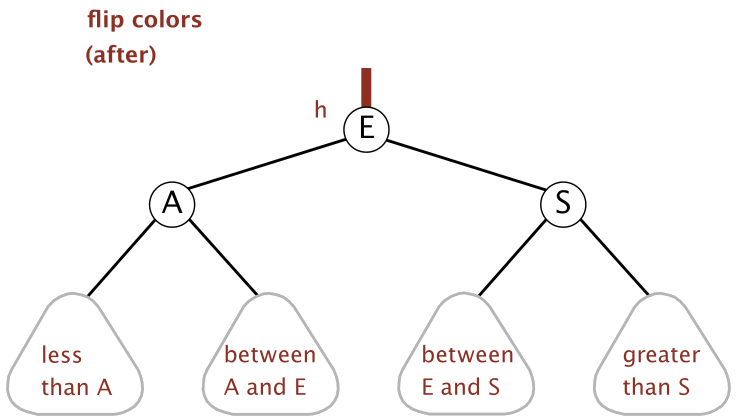
\includegraphics[width=.9\textwidth]{img/red_black_colo_flip_after.png}
        \caption{Fonte: \cite{sedgewick2014algorithms}}
      \end{figure}
    \end{column}
  \end{columns}

  \tcb{Invariantes:} Manter ordem simétrica e balanceamento perfeito de arestas pretas.

\end{frame}

\begin{frame}[fragile,t]
  \frametitle{Operações elementares de Árvores RB}

  \tcb{Color flip} Recolorir um nó-4 temporário para dividi-lo.

      \begin{minted}[frame=lines,framesep=2mm,baselinestretch=1,fontsize=\small,linenos]{c}
ArvoreRB * flip_cor(ArvoreRB * no){
  no->cor = RED;
  no->esq->cor = BLACK;
  no->dir->cor = BLACK;
  return(x);
}
      \end{minted}

  \tcb{Invariantes:} Manter ordem simétrica e balanceamento perfeito de arestas pretas.

\end{frame}

\section{Inserção em Árvores Red-Black}

\begin{frame}
  \frametitle{Inserção Árvores RB}

  \tcb{Aquecimento 1:} Inserir em uma árvore com um único no.

  \begin{figure}[h]
    \centering
    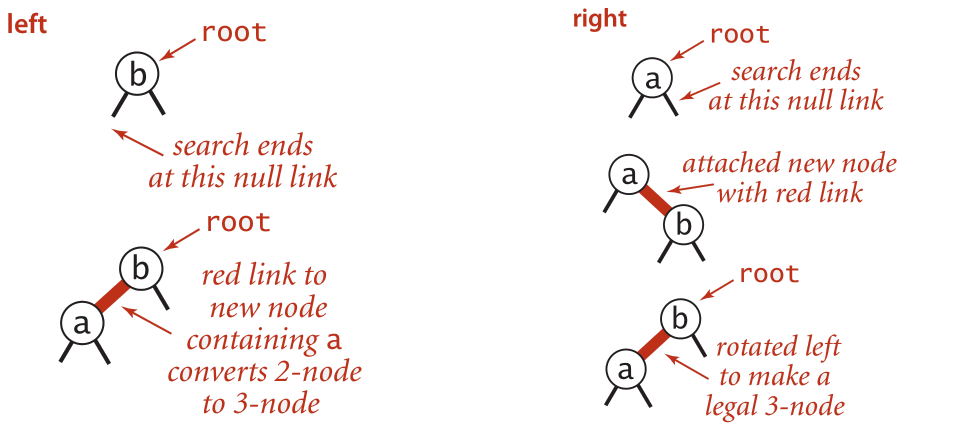
\includegraphics[width=\textwidth]{img/red_black_insert_1_node.png}
    \caption{Fonte: \cite{sedgewick2014algorithms}}
  \end{figure}

\end{frame}

\begin{frame}
  \frametitle{Inserção Árvores RB}

  \small{
  \tcb{Caso 1:} Inserir em um nó-2 folha.
  \begin{itemize}
    \item Inserção normal de árvore binária; nova aresta é vermelha;
      \textcolor{gray}{\scriptsize{para manter ordem simétrica e balanceamento perfeito de arestas pretas}}
    \item Se a nova aresta vermelha descende à direita, rotaciona para esquerda.
      \textcolor{gray}{\scriptsize{para corrigir o invariante das cores}}
  \end{itemize}
}

  \begin{figure}[h]
    \centering
    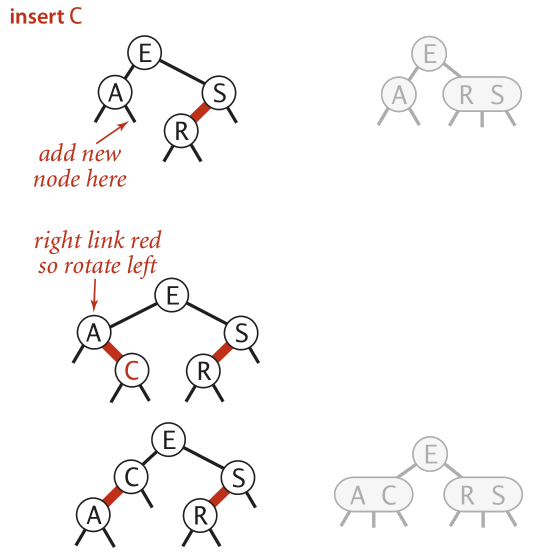
\includegraphics[width=.5\textheight]{img/red_black_insert_case_1.png}
    \caption{Fonte: \cite{sedgewick2014algorithms}}
  \end{figure}

\end{frame}

\begin{frame}
  \frametitle{Inserção Árvores RB}

  \tcb{Aquecimento 2:} Inserir em uma árvore com exatamente 2 nós.

  \begin{figure}[h]
    \centering
    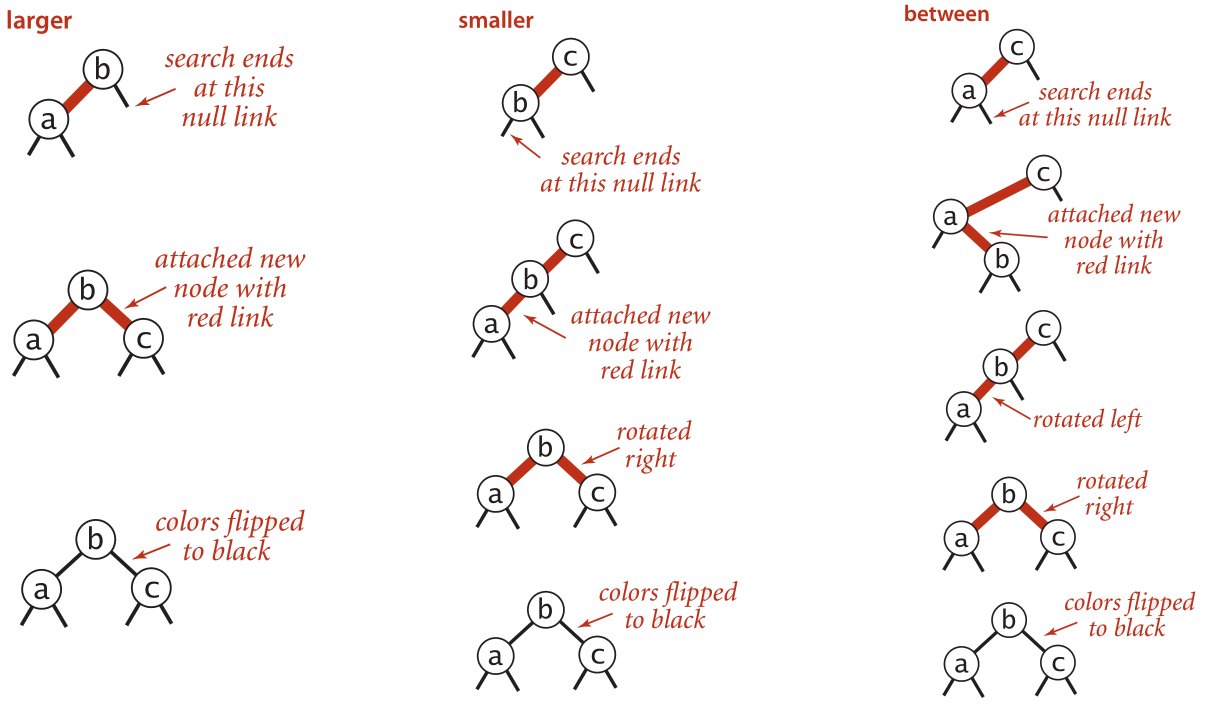
\includegraphics[width=\textwidth]{img/red_black_insert_warmup_2.png}
    \caption{Fonte: \cite{sedgewick2014algorithms}}
  \end{figure}

\end{frame}

\begin{frame}
  \frametitle{Inserção Árvores RB}

  \small{
  \tcb{Caso 2:} Inserir em um nó-3 folha.
  \begin{itemize}
    \item Inserção normal de árvore binária; nova aresta é vermelha;
      \textcolor{gray}{\scriptsize{para manter ordem simétrica e balanceamento perfeito de arestas pretas}}
    \item Rotaciona para balancear o nó-4 temporário (se necessário);
    \item Trocar cores para passar a aresta vermelha para o nível acima;
    \item Rotacionar para aresta vermelha descender para esquerda (se necessário);
      \textcolor{gray}{\scriptsize{para corrigir o invariante das cores}}
  \end{itemize}
}

  \begin{figure}[h]
    \centering
    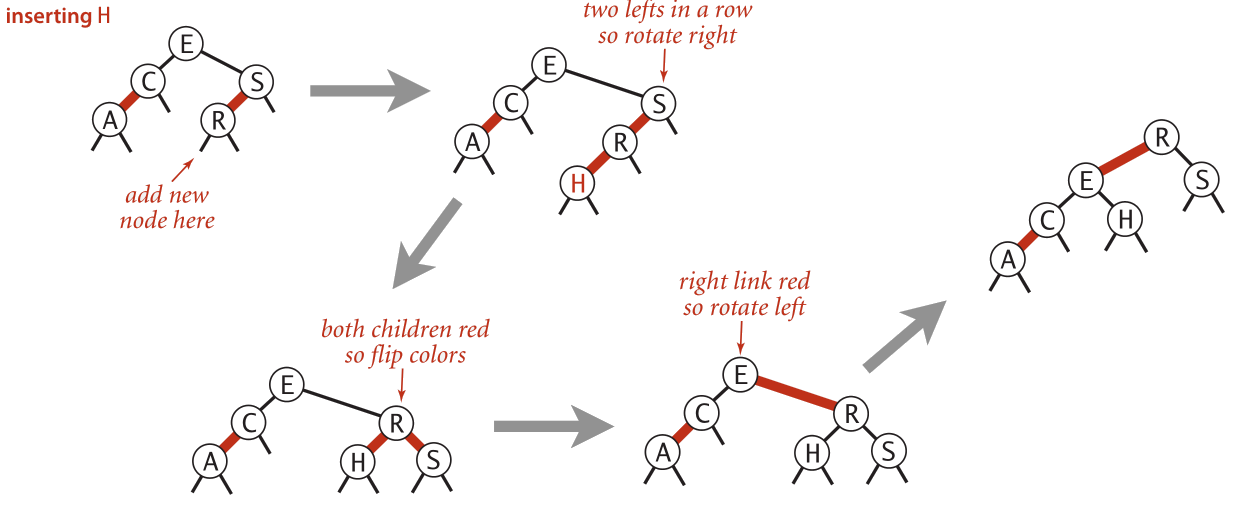
\includegraphics[width=.8\textwidth]{img/red_black_insert_case_2.png}
    \caption{Fonte: \cite{sedgewick2014algorithms}}
  \end{figure}

\end{frame}

\begin{frame}
  \frametitle{Inserção Árvores RB}

  \tcb{Finalização:} Se necessário, repita casos 1 e 2 nos níveis anteriores da árvore.

  \begin{figure}[h]
    \centering
    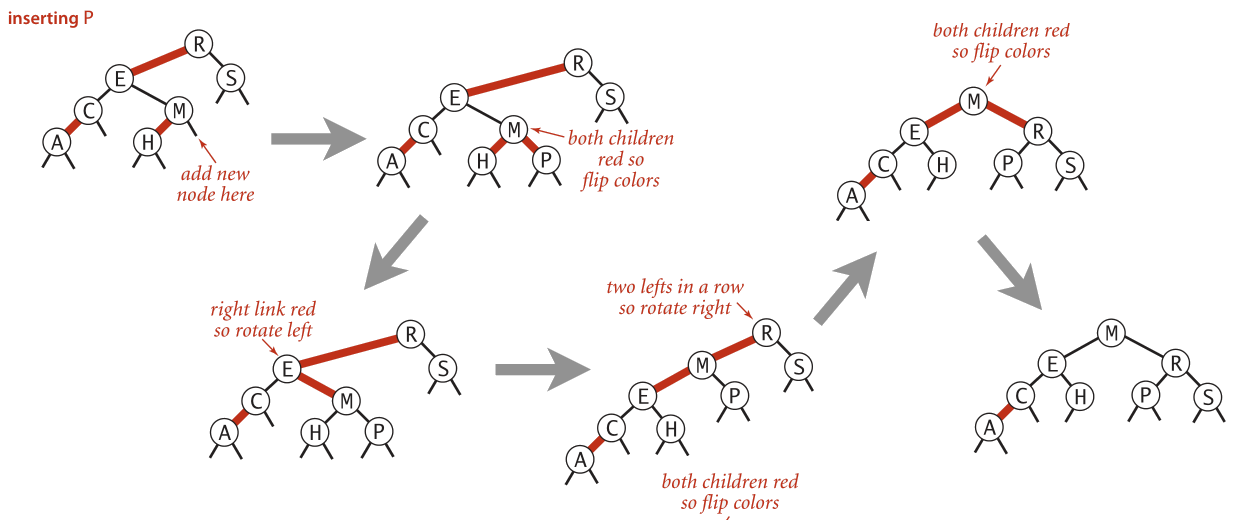
\includegraphics[width=\textwidth]{img/red_black_insert_up_tree.png}
    \caption{Fonte: \cite{sedgewick2014algorithms}}
  \end{figure}

\end{frame}

\begin{frame}[t]
  \frametitle{Inserção Árvore RB - Exemplo}

  \begin{columns}
    \begin{column}{0.5\textwidth}
      \begin{figure}[h]
        \centering
        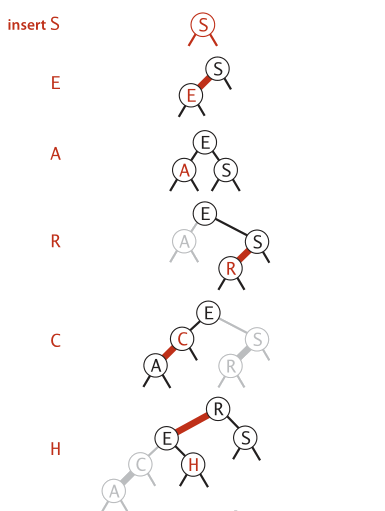
\includegraphics[width=.9\textwidth]{img/red_black_insert_ex_1_1.png}
      \end{figure}
    \end{column}
    \begin{column}{0.5\textwidth}
      \begin{figure}[h]
        \centering
        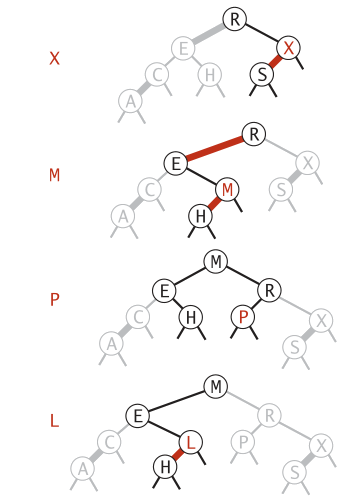
\includegraphics[width=.85\textwidth]{img/red_black_insert_ex_1_2.png}
        \caption{Fonte: \cite{sedgewick2014algorithms}}
      \end{figure}
    \end{column}
  \end{columns}

\end{frame}

\begin{frame}[t]
  \frametitle{Inserção Árvore RB - Exemplo ordem crescente}

  \begin{columns}
    \begin{column}{0.5\textwidth}
      \begin{figure}[h]
        \centering
        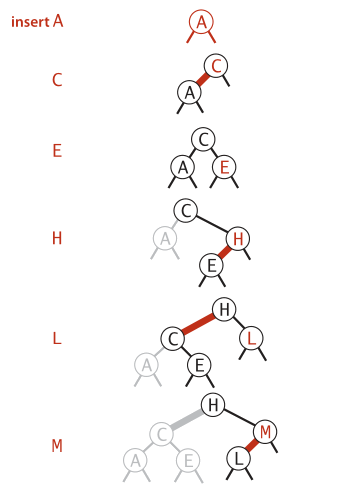
\includegraphics[width=.75\textwidth]{img/red_black_insert_ex_2_1.png}
      \end{figure}
    \end{column}
    \begin{column}{0.5\textwidth}
      \begin{figure}[h]
        \centering
        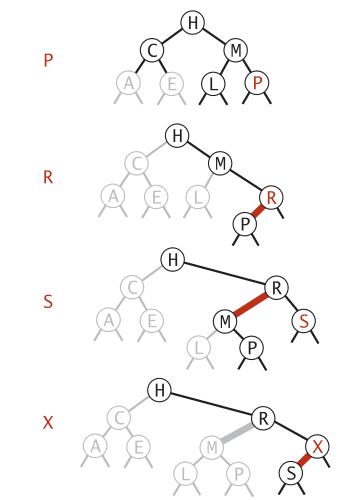
\includegraphics[width=.85\textwidth]{img/red_black_insert_ex_2_2.png}
        \caption{Fonte: \cite{sedgewick2014algorithms}}
      \end{figure}
    \end{column}
  \end{columns}

\end{frame}

\begin{frame}
  \frametitle{Inserção: implementação}

  \smaller{
  \tcb{Mesmo código para todos os casos}
  \begin{itemize}
    \item Filho à direita vermelho, filho à esquerda preto: \tcr{rotaciona à esquerda};
    \item Filho à esquerda vermelho, neto à esquerda vermelho: \tcr{rotaciona à direita};
    \item Ambos filhos vermelhos: \tcr{troca cores};
  \end{itemize}
  }
  
  \begin{figure}[h]
    \centering
    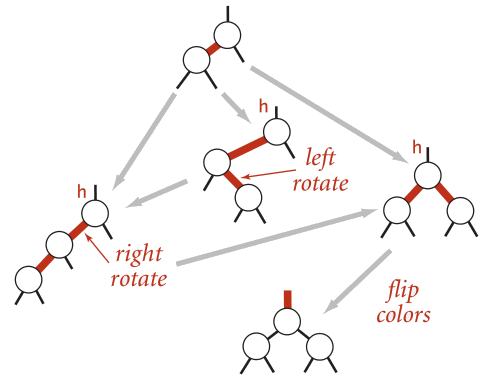
\includegraphics[width=.65\textwidth]{img/red_black_insert_implementation.png}
    \caption{Fonte: \cite{sedgewick2014algorithms}}
  \end{figure}
\end{frame}

\begin{frame}
  \frametitle{Exemplos}

  \begin{figure}[h]
    \centering
    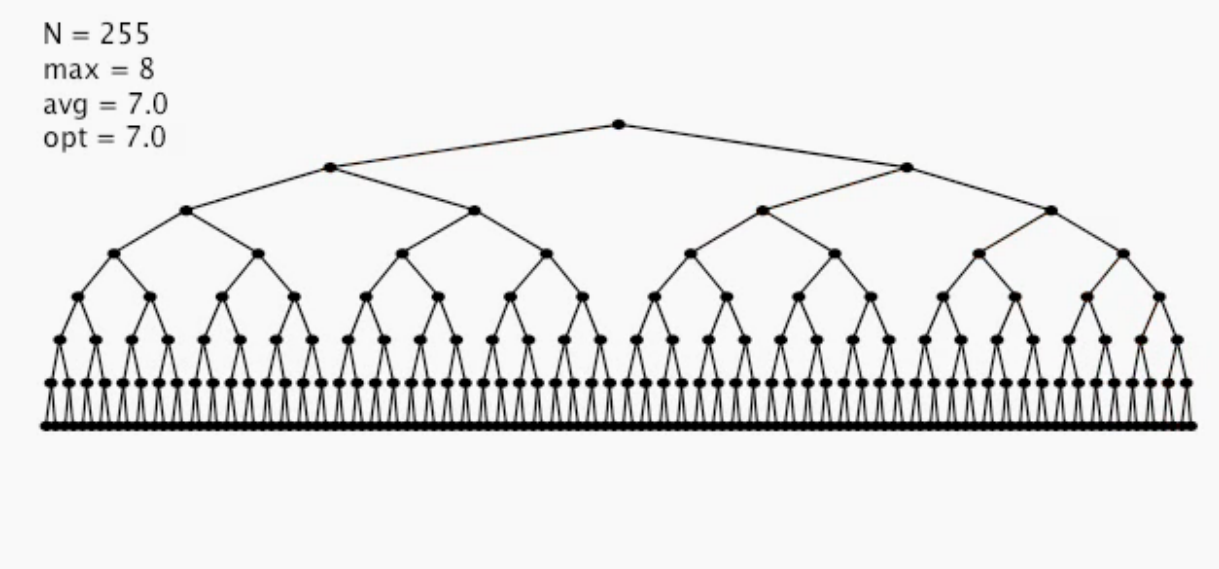
\includegraphics[width=\textwidth]{img/red_black_example_ascending.png}
    \caption{255 inserções em ordem crescente.\\Fonte: \cite{sedgewick2014algorithms}}
  \end{figure}
\end{frame}

\begin{frame}
  \frametitle{Exemplos}

  \begin{figure}[h]
    \centering
    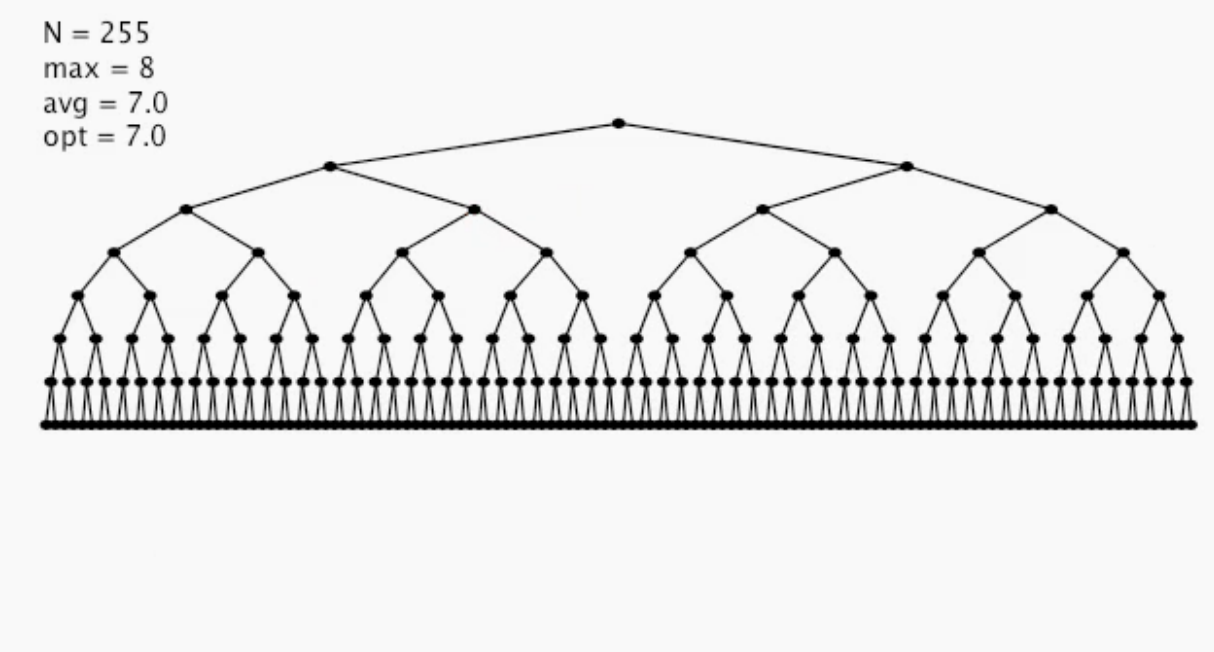
\includegraphics[width=\textwidth]{img/red_black_example_descending.png}
    \caption{255 inserções em ordem decrescente.\\Fonte: \cite{sedgewick2014algorithms}}
  \end{figure}
\end{frame}

\begin{frame}
  \frametitle{Exemplos}

  \begin{figure}[h]
    \centering
    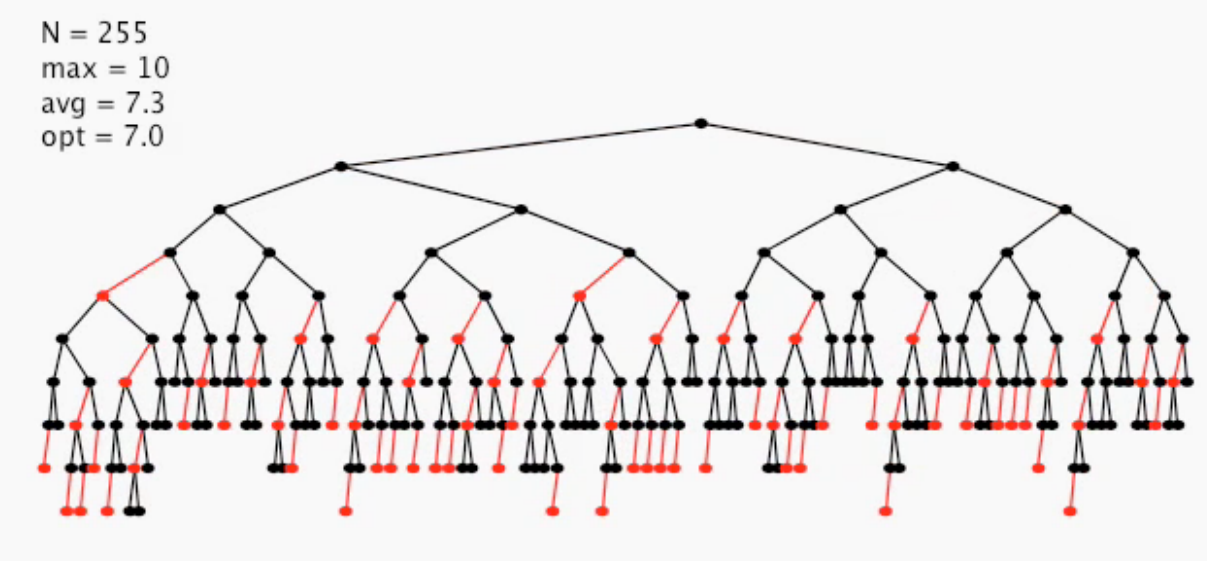
\includegraphics[width=\textwidth]{img/red_black_example_random.png}
    \caption{255 inserções em ordem aleatória.\\Fonte: \cite{sedgewick2014algorithms}}
  \end{figure}
\end{frame}

\begin{frame}
  \frametitle{Desempenho}

  \tcb{Proposição} Altura da árvore é $\le 2 \log_{2}{N}$ no pior caso.
  \begin{itemize}
    \item Todos os caminhos da raiz até as folhas tem o melhor número de arestas pretas;
    \item Nunca existem duas arestas vermelhas em sequência.
  \end{itemize}

  \begin{figure}[h]
    \centering
    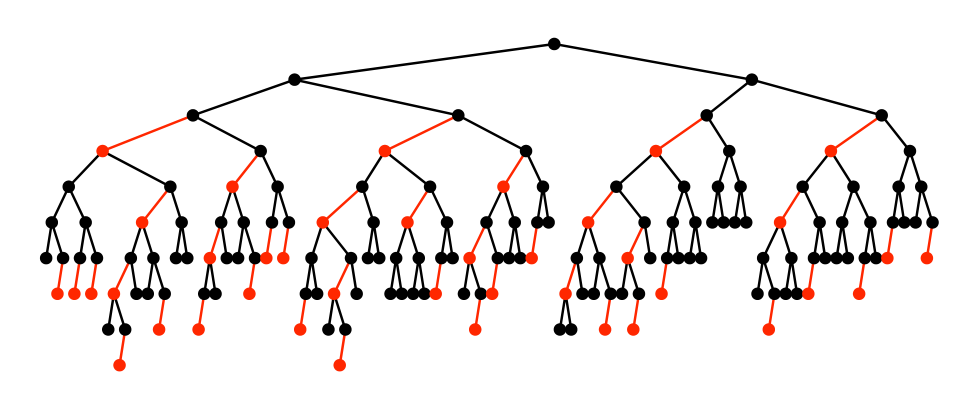
\includegraphics[width=.7\textwidth]{img/red_black_performance.png}
    \caption{Fonte: \cite{sedgewick2014algorithms}}
  \end{figure}

  \tcb{Propriedade} Altura da árvore é $\sim 1.0 \log_{2}{N}$ em aplicações típicas.


\end{frame}

\begin{frame}
  \frametitle{Resumo Implementações Tabela de Símbolos}

  \begin{figure}[h]
    \centering
    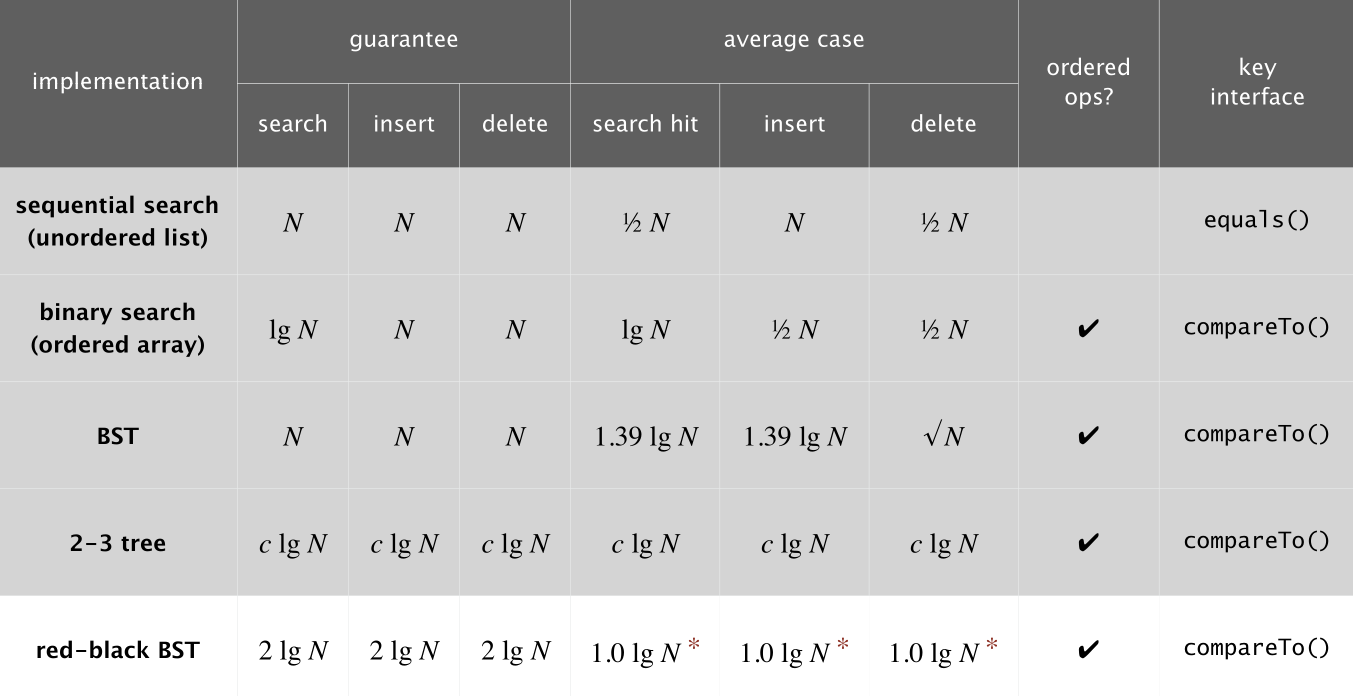
\includegraphics[width=\textwidth]{img/symbol_table_review_3.png}
    \caption{Fonte: \cite{sedgewick2014algorithms}}
  \end{figure}

  \scriptsize{* valor exato do coeficiente não é conhecido, mas é extremamente próximo de 1}


\end{frame}

% ========================================== 
% Frame para referências 
\begin{frame}[allowframebreaks] 
  \frametitle{Referências utilizadas na apresentação}
  \bibliography{referencias}
\end{frame}
% ==========================================

\end{document}
